% !TEX root = ../main.tex
\section{Challenges}
\label{sec:problem}

\begin{figure}
\centering
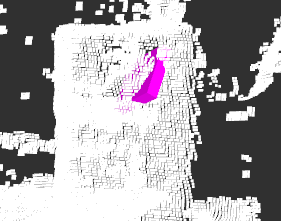
\includegraphics[width=\columnwidth]{figs/mismatch_tag}
\caption{Close up snapshot on the rectangular prism. The physical tag is placed on the surface of the prism but the detected tag is oriented into the prism.}
\label{fig:mismatch}
\end{figure}
In square fiducial marker detection, the pose is calculated by using the four corners of the tag. Since the tags are planar, it is easy to compute perspective point correspondences from the corners. This can be formalized as a specific case of the Perspective-N-Point problem and it has been well studied in geometry based Computer Vision literatures \citep{hartley2003multiple, zhang2005general}. There are numerous optimization methods such as ones proposed in \citep{dementhon1992exact} and \citep{haralick1994review} to solve this problem. In particular, in \citep{horaud1989analytic}, the author shows that there is a deterministic solution to the Perspective-4-Point (P4P) problem when the points are coplanar. In other words, given the projection of a tag's four corners, the pose of the tag is unique. In practice, however, this method is very sensitive to noise. When ARTags, Apriltags and ARToolkit systems are used in scenarios shown in Figure \ref{fig:table_clearing}, the poses of the tags are unstable even when the scene is static. Since the minimal number of perspective points are used to estimate the pose, a small variance in the corner detection process will yield estimations far from the true pose, as shown in Figure \ref{fig:mismatch}.

We will illustrate an ambiguity effect caused by noise by using two over lapping cubes, shown in Figure \ref{fig:cube}. The overlapping face of the two cubes are interlaced but rotated by 120 degrees. However, due to perspective projection, the squares appear to be on the same plane. With low camera resolution, the overlapping squares become virtually indistinguishable. The red circular regions are the detected corners under some sensory noise. Even though the reprojection error is minimized in the 2D space using P4P optimization methods, the 3D pose can still be far off. The result of the optimization can be characterized as a bimodal distribution and a function of the the viewing angle. Depending on the noise level in the scene, the optimization might converge to either one of the local minima causing the pose estimation to be unreliable.

\begin{figure}
\centering
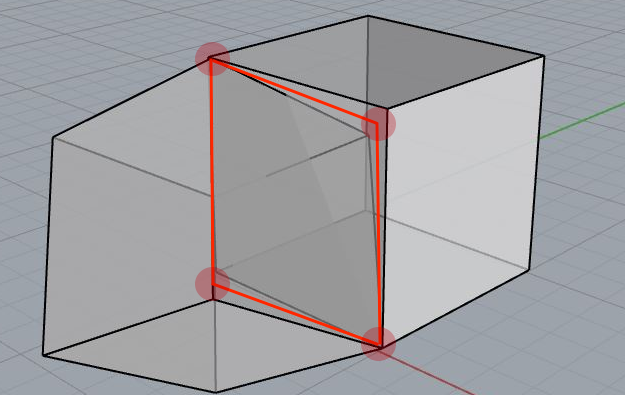
\includegraphics[width=\columnwidth]{figs/perspective_fig}
\caption{The ambiguity effect is illustrated with two rendered cubes in the perspective view. The two cubes are rotated such that two faces are interlaced. The red square is a simulated projection of a square tag. The red circular regions denote the region of potential corner detections in a noisy scene. The pose of the red square can converge to either one of the two faces.}
\label{fig:cube}
\end{figure}